\documentclass[12pt,a4paper]{article}
\usepackage[english]{babel}
\usepackage[utf8]{inputenc}
\usepackage{amssymb,amsmath}
\usepackage[all]{xy}
\usepackage{url}
\usepackage{graphicx}
\usepackage{color}
\newcommand{\angstrom}{\textup{\AA}}
\color{black}
\usepackage{geometry}
\usepackage[autostyle]{csquotes}
\usepackage{tikz}
\usetikzlibrary{bayesnet}
\usepackage{dcolumn}
\usepackage{booktabs}
\usepackage{tikz}
\usetikzlibrary{positioning,shapes,arrows}
\newcolumntype{M}[1]{D{.}{.}{1.#1}}

\geometry{
	a4paper,
 	left=15mm,
 	right=15mm,
 	top=10mm,
 	bottom=15mm
}


\begin{document}
\title{Venice Boat Classification}
\author{Michał Ostyk-Narbutt, 1854051 \\ \\ Prof. Iocchi, Machine Learning Homework 2 \\  La Sapienza University of Rome}

\maketitle
\tableofcontents
\clearpage
\section{Introduction}

This report describes two approaches to tacking the problem of classifying boats seen in the Venice Grand Canal. The first on being by training a self-made convolutional neural network (CNN), whereas the latter using a pre-trained network VGG16 and extracting the bottleneck features in order to train a Support Vector Machine (SVM). Both classifiers give promising results based on the imbalanced nature of the dataset.
\section{Experimental Data}
The data used was taken from the Sapienza University Lab Rococo website. It consisted of over 5000 images belonging to 24 different classes. However, due to the fact that only 18 appeared in both the training and testing set, the non-appearing six were discarded from further analysis. Moreover, the dataset is heavily imbalanced with only 7 classes having over 50 samples.

Each image in the dataset had the dimensions of $ 240 \times 800 \times 3$ with the $3$ depicting the very important RGB nature of each image.
\section{Tools and methodology}
\subsection{Tools}
To perform classification using both methods, I used the programming language Python along with two key libraries for deep learning and machine learning: \texttt{Keras} and \texttt{Scikit-learn}. The specific requirements are listed in the \texttt{requirement.txt} file  of the code.

\subsection{methodology}
\subsubsection{preprocessing}
Before being to train the dataset and achieve any results, preprocessing was a necessary step. It concluded of discarding 6 classes which do not appear in the training set, and piling them up into a tree structure where every image of each class appeared in a separate folder whose name was that specific class. This latter step is a requirement made by the framework deep learning framework.\\
The subsequent steps were taken separately for the two methods used:
\begin{itemize}
\item \texttt{VGCC18} $-$ Venice Grand Canal Classifier 2018 
\item \texttt{VGG16+SVM} 
\end{itemize}
\subsection{VGCC18}
The Venice Grand Canal Classifier 2018 is a CNN made espcially for the purposes of classifying boats in Venice. It consists of 
\begin{itemize}
\item 3  convolutional layers, each activated by the ReLU function, and followed by dropout of probability $=0.2$ 
\item One fully connected layer also activated by the ReLU function, and followed by dropout of probability $=0.6$ 
\item One output softmax layer of size 18 which is equal to the number of classes which gives the probability of each class.
\end{itemize}
The images were rescaled to size $=200 \times 200$ to reduce the number of parameters which could avoid overfitting and help ease training time.The were also subject to random rotations of 30 degrees, rescaling, zooming in and horizontal flipping during training.

Prior training, the a part of the training set was set aside to become the validation set in order to track progress during the training. This is important to see that the network does not overfit and learn unnecessary features only seen in the training set.

\subsection{VGG16+SVM}
In this part, the famoues VGG16 convolutional network was used which was pre-trained on the massive imagenet dataset. This dataset includes very generic pictures of everyday objects, but it also contains, ships and boats. This feature is useful for classifying very specific types of boats mainly seen only in Venice, Italy. This method is compromised of the following steps, extracting the specific features of the 2nd conv layer of VGG16, and training a generic SVM on them. In order to complete this step, the images were rescaled to fit the pre-trained network to size $=224 \times 224$.


\section{Results}
\subsection{VGCC18}
The network was trained on 10 epochs, with the default Keras batch size of 32. 2510 were part of the training set, wheras 1300 were part of the validation set. The figure below depicts the accuracy and loss during training at each epoch.

\begin{figure}[htbp]
\begin{center}
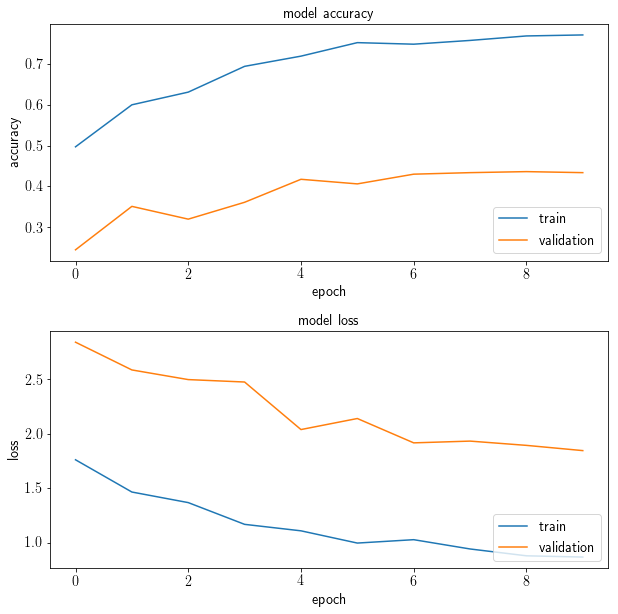
\includegraphics[width=0.75\columnwidth, angle = 0]{img/vgcc18.png}
\end{center}
\caption{The accuracy and log loss for both training and validation sets at each epoch.}
\label{img:1roc1}
\end{figure}
As Figure 1 depicts, the validation accuracy is much smaller than the training accuracy but rises with each epoch as does the training. This can be partly due to the fact that the validation set contained very few examples, but the relatively steady rise, does not lead one to infer massive overfitting.

The final accuracy on the test set of 1252 images was: $68.9 \%$
\subsection{VGG16+SVM}

Upon extracting the CNN codes from VGG16, the images were transformed using Principal Component analysis to reduce the feature space. Standard scaling did not improve results. This may be due to the similar nature of all the classes with surrounding water around each boat. The SVM was trained on 3810 images, and tested on the remaining 1252 images. 

The results are as follows:

\begin{table}[h]
\begin{tabular}{|c|c|c|}
\hline
SVM type           & Accuracy & Kernel \\ \hline
Linear SVC         & $18 \%$  & linear \\ \hline
SVC + kernel trick & $24 \%$  & RBF    \\ \hline
\end{tabular}
\end{table}

\section{Conclusions}
To sum up,only the \texttt{VGCC18} approach to classifying the boats in the Venice Grand Canal, which yielded an accuracy of $69\%$ gave promising results. On the other hand, training an SVM on top of CNN codes extracted from a pre-trained network gave quite poor results but given the nature of the dataset which is heavily imbalanced, these results cannot be deemed irrelevant . Both the Linear SVC and SVC with the kernel trick gave accuracies $18 \%$ and $24 \%$ respectively. The score could be improved with using a better pre-trained CNN to extract features and perhaps from a different layer. The score of the first method could be improved by stacking more convolutional layers, and creating more instances but it would come at an expense of time and computational power, which is scarce.

\end{document}
